% ============================================================
%  深圳大学实验报告模板(SZU Experiment Report Template)
% This template can be modified according to the specific requirements of your experiment or project.
% Produced by: Chao Fan and Kewei Ou, AI School of SZU
% ============================================================

\documentclass[a4paper,12pt]{article}

% ----------------------------
% 中文与字体支持
% ----------------------------
\usepackage{fontspec}    % 字体支持
\usepackage{xeCJK}       % 中文字体支持
\setCJKmainfont{Noto Serif CJK SC} % 设置中文字体(Overleaf自带Noto字体)

% ----------------------------
% 页面设置与常用宏包
% ----------------------------
\usepackage{geometry}    % 页面边距控制
\geometry{left=1in, right=1in, top=1in, bottom=1in}

\usepackage{longtable}   % 支持长表格
\usepackage{graphicx}    % 插入图片
\usepackage{fancyhdr}    % 页眉页脚控制
\usepackage{tikz}        % 绘制框线等图形
\usetikzlibrary{calc}    % 坐标计算
\usepackage{verbatim}    % 显示代码块
\usepackage{float}       % 控制图片浮动位置([H]参数)

% ----------------------------
% 页眉页脚设置
% ----------------------------
\pagestyle{fancy}
\fancyhf{} % 清空默认页眉页脚
\fancyhead[L]{深圳大学实验报告} % 左侧页眉文字
\fancyhead[C]{} % 中间空
\fancyhead[R]{} % 右侧空

% ============================================================
%                      文档开始
% ============================================================

\begin{document}

% ============================================================
% 封面页
% ============================================================
\begin{titlepage}
    \centering
    \vspace*{2cm}
    \Huge{\textbf{深 \ 圳 \ 大 \ 学 \ 实 \ 验  \ 报 \ 告}}\\[1.5cm]
    
    \Large{课程名称:\underline{\hspace{8cm}}}\\[0.5cm]
    \Large{项目名称:\underline{\hspace{8cm}}}\\[0.5cm]
    \Large{学 \quad \quad 院:\underline{\hspace{8cm}}}\\[0.5cm]
    \Large{专 \quad \quad 业:\underline{\hspace{8cm}}}\\[0.5cm]
    \Large{指导教师:\underline{\hspace{8cm}}}\\[0.5cm]
    \Large{报告人:\underline{\hspace{3cm}} \hspace{0.5cm} 学号:\underline{\hspace{3cm}}}\\[0.5cm]
    \Large{实验时间:\underline{\hspace{8cm}}}\\[0.5cm]
    \Large{提交时间:\underline{\hspace{8cm}}}\\[1.5cm]

    \vfill
    \Large{教务处制}
\end{titlepage}

\newpage

% ============================================================
% 正文部分
% ============================================================
% Experiment Objectives


\section{Objectives}

Describe the goal of the experiment, including what you aim to achieve (e.g., testing an algorithm, solving a problem, or exploring a concept).


% Experiment Process
\section{Overview}
Briefly outline the approach and methods used in the experiment.
\begin{enumerate}
    \item[Spot 1]: xxx;
    \item[Spot 2]: xxx;
    \item[Spot 3]: xxx;
\end{enumerate}

% Figure
\begin{figure}[t]
    \centering
    \includegraphics[width=0.92\linewidth]{figs/vit_overview.png}
    \caption{xxx}
    \label{fig:vit-arch}
\end{figure}

% Implementation Details
\section{Implementations}
Provide a high-level overview of the key parts of your code.

As shown in Figure.~\ref{fig:vit-arch}, xxx: 
\begin{enumerate}
    \item[Part 1]: xxx;
    \item[Part 2]: xxx;
    \item[Part 3]: xxx;
\end{enumerate}

\section{Results}

Present the output generated by your program. 
Include any test cases, screenshots, or tables of results.

\section{Discussion}

Analyze the performance of your program. 
Discuss any errors, inefficiencies, or areas for improvement. 

\newpage

% ============================================================
% 批阅与成绩评定页
% ============================================================

% 绘制正文外框(包含批阅区域)
\begin{tikzpicture}[remember picture, overlay]
  \draw[thick] 
    ($(current page.north west)+(2cm,-3cm)$) 
    rectangle 
    ($(current page.south east)+(-2cm,2.5cm)$);
\end{tikzpicture}

\vspace{1cm}

% 批阅区
\noindent \textbf{指导教师批阅意见:}
\vspace{5cm}
\hfill

\vspace{1cm}

\noindent \textbf{成绩评定:}
\vspace{2cm}
\hfill

\vspace{1cm}

\noindent \textbf{指导教师签字:}
\vspace{2cm}
\hfill

\vspace{1cm}

% 备注部分
\noindent \textbf{备注:}
\begin{itemize}
    \item 报告内的项目或内容设置,可根据实际情况加以调整和补充。
    \item 教师批改学生实验报告时间应在学生提交实验报告时间后 10 日内。
\end{itemize}

% ============================================================
%                      文档结束
% ============================================================

\end{document}